\chapter{Implementación y Mediciones}

\section{Identificación de pines}
\begin{table}[H]
\centering
\renewcommand{\arraystretch}{1.8}
\begin{tabular}{|m{4cm}|m{2cm}|m{2cm}|m{2cm}|m{2cm}|}
\hline

\multirow{2}{*}{
\begin{tabular}{c}
Sentido de las puntas \\del multímetro
\end{tabular}
}
&
\multicolumn{2}{c|}{Diodo de germanio} & \multicolumn{2}{c|}{Diodo de silicio}\\
\cline{2-5}
& D1 & D2 & D1 & D2 \\
\hline
\centering\includegraphics[width=2.5cm]{img/tester-diodo-dir.png}
& 324\,mV & 294\,mV & 598\,mV & 613\,mV\\
\hline
\centering\includegraphics[width=2.5cm]{img/tester-diodo-inv.png}
& OL & OL & OL & OL \\
\hline
\end{tabular}
\caption{Mediciones con el multímetro en diferentes polaridades}
\label{tab:mediciones_diodos}
\end{table}



\begin{figure}[H]
\centering

\begin{minipage}{0.45\textwidth}
    \centering
    \includegraphics[height=7cm]{img/tester-1N4007-dir.jpeg}
    \caption{Medición en directa}
\end{minipage}
\hspace{0.02\textwidth}
\begin{minipage}{0.45\textwidth}
    \centering
    \includegraphics[height=7cm]{img/tester-1N4007-inv.jpeg}
    \caption{Medición en inversa}
\end{minipage}
\end{figure}

Las mediciones realizadas con el multímetro permitieron identificar la polaridad y el tipo de conducción de los diodos. Cuando las puntas se conectaron en polarización directa, el diodo de germanio presentó una 
caída de tensión cercana a 0.3V, mientras que el diodo de silicio mostró valores alrededor de 0.6V. En cambio, al invertir las puntas del multímetro, ambos diodos indicaron “OL”, mostrando que en polarización inversa prácticamente no conducen corriente.


\section{Curva características de los diodos}

\begin{figure}[H]
    \centering
    \includegraphics[width=0.7\textwidth]{img/Circuito-básico-diodo-directa.png}
    \caption{}
    \label{fig:circuito-básico-mediciones}
\end{figure}


\subsection{Mediciones Circuito Básico con 1N4007}

\begin{table}[H]
\centering
\resizebox{\textwidth}{!}{
\begin{tabular}{|c|c|c|c|c|c|>{\columncolor{gray!30}}c|c|c|c|c|c|c|c|}
\hline
\multicolumn{14}{|c|}{1N4007} \\
\hline
V1 & 0 & 0,1 & 0,3 & 0,4 & 0,45 & 0,5 & 0,55 & 0,6 & 0,65 & 0,7 & 1 & 3 & 5 \\
\hline
V1(real) [V]
& 0& 0,1& 0,326& 0,395& 0,46& 0,512& 0,567& 0,612& 0,654& 0,712& 1,01& 3,062& 5,02 \\
\hline
VD [V]
& 0& 0,1& 0,322& 0,389& 0,429& 0,470& 0,491& 0,506& 0,507& 0,53& 0,571& 0,657& 0,686 \\
\hline
ID [mA]
& 0& 0& 0& 0& 0,016& 0,030& 0,066& 0,094& 0,122& 0,163& 0,398& 2,4& 4,33 \\
\hline

\end{tabular}}
\caption{Mediciones del diodo 1N4007}
\end{table}

\begin{figure}[H]
    \centering
    \includegraphics[width=0.9\textwidth]{img/mediciones-testers(3)-1N4007.jpeg}
    \caption{Mediciones para una alimentación de 0.512 V}
    \label{fig:mediciones-testers(3)-1N4007}
\end{figure}

\begin{figure}[H]
\centering

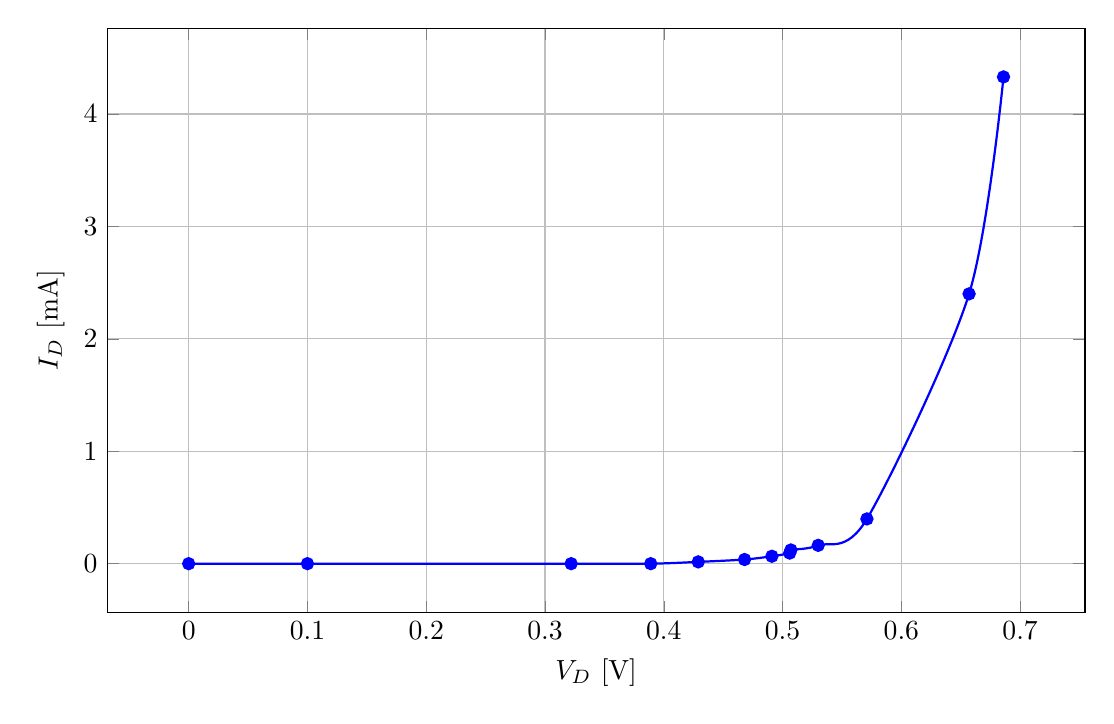
\begin{tikzpicture}
\begin{axis}[
    width=14cm,
    height=9cm,
    xlabel={$V_D$ [V]},
    ylabel={$I_D$ [mA]},
    grid=major,
    smooth,
    mark=*,
]
\addplot [
    color=blue,
    thick,
    mark=*,
]
coordinates {
(0,0)
(0.1,0)
(0.322,0)
(0.389,0)
(0.429,0.016)
(0.468,0.037)
(0.491,0.066)
(0.506,0.094)
(0.507,0.122)
(0.53,0.163)
(0.571,0.398)
(0.657,2.4)
(0.686,4.33)
};
\end{axis}
\end{tikzpicture}
\caption{Característica $I_D(V_D)$ del diodo 1N4007}
\label{fig:idvd_1n4007}
\end{figure}

\subsection{Mediciones Circuito Básico con 1N60}

\begin{table}[H]
\centering
\small
\resizebox{\textwidth}{!}{
\begin{tabular}{|c|c|c|c|c|c|c|c|c|c|c|c|c|>{\columncolor{gray!30}}c|}
\hline
\multicolumn{14}{|c|}{1N60} \\
\hline
V1 [V]
& 0& 0,1& 0,15& 0,2& 0,25& 0,3& 0,35& 0,4& 0,5& 0,7& 1& 3& 5 \\
\hline
V1(real) [V]
& 0& 0,107& 0,152& 0,218& 0,244& 0,297& 0,355& 0,408& 0,514& 0,695& 1,015& 3,038& 5,05 \\
\hline
VD [V]
& 0& 0,091& 0,118& 0,146& 0,155& 0,17& 0,185& 0,196& 0,216& 0,245& 0,295& 0,496& 0,653 \\
\hline
ID [mA]
& 0& 0,012& 0,03& 0,064& 0,08& 0,133& 0,152& 0,191& 0,268& 0,407& 0,659& 2,54& 4,4 \\
\hline

\end{tabular}
}
\caption{Mediciones del diodo 1N60}
\end{table}

\begin{figure}[H]
    \centering
    \includegraphics[width=0.9\textwidth]{img/mediciones-testers(3)-1N60.jpeg}
    \caption{Mediciones para una alimentación de 5.05 V }
    \label{fig:mediciones-testers(3)-1N60}
\end{figure}

\begin{figure}[H]
\centering
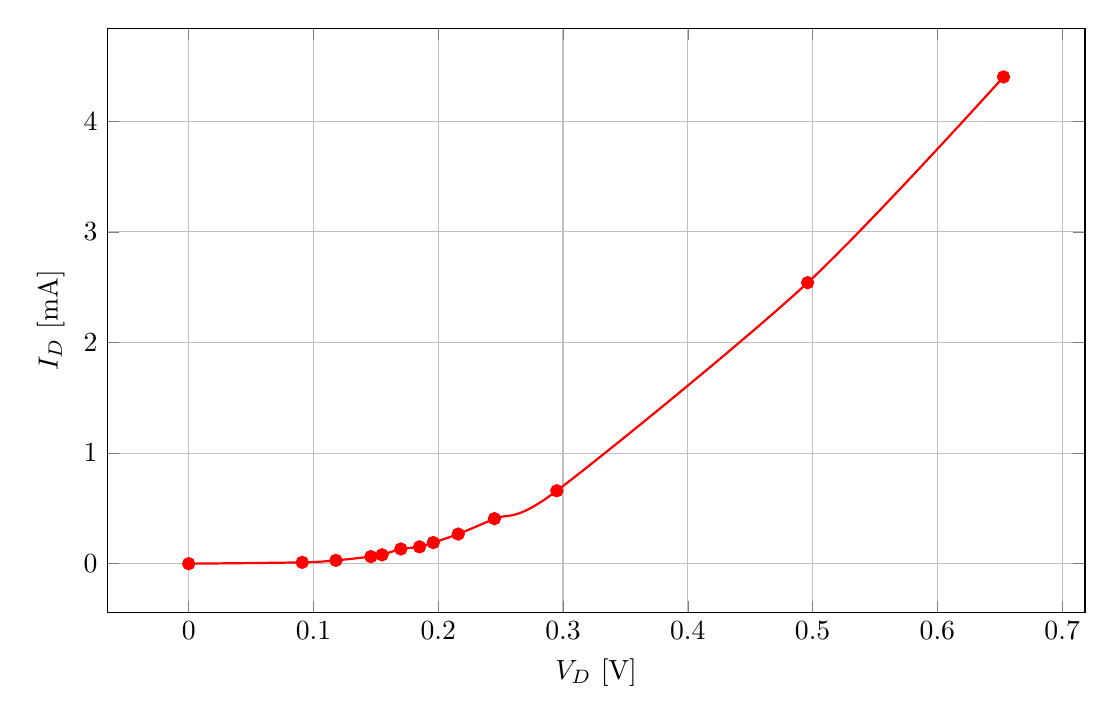
\begin{tikzpicture}
\begin{axis}[
    width=14cm,
    height=9cm,
    xlabel={$V_D$ [V]},
    ylabel={$I_D$ [mA]},
    grid=major,
    smooth,
    mark=*,
]
\addplot [
    color=red,
    thick,
    mark=*,
]
coordinates {
(0,0)
(0.091,0.012)
(0.118,0.03)
(0.146,0.064)
(0.155,0.08)
(0.17,0.133)
(0.185,0.152)
(0.196,0.191)
(0.216,0.268)
(0.245,0.407)
(0.295,0.659)
(0.496,2.54)
(0.653,4.4)
};
\end{axis}
\end{tikzpicture}
\caption{Característica $I_D(V_D)$ del diodo 1N60}
\label{fig:idvd_1n60}
\end{figure}

A partir de las mediciones realizadas se obtuvieron las características $I_D(V_D)$ de los diodos 1N4007 y 1N60. 
En ambos casos se observa que, para bajas tensiones directas, la corriente permanece prácticamente nula. Sin embargo, al aumentar la tensión aplicada, la corriente comienza a incrementarse rápidamente, evidenciando 
el comportamiento no lineal característico de los diodos.

El diodo 1N60 no presenta una caída de tensión fija en 0.3V, ya que dicho valor es solamente aproximado. Al ser un diodo de germanio, comienza a conducir con tensiones menores y su tensión directa varía considerablemente con la corriente. 
En cambio, el 1N4007, al ser de silicio, posee una conducción más marcada alrededor de 0.7V, por lo que su caída de tensión se mantiene más cercana a ese valor en condiciones normales de funcionamiento.

\section{Circuitos recortadores con diodos zener}


En esta sección se implementaron físicamente sobre una protoboard los circuitos recortadores previamente simulados en LTspice, con el objetivo de comparar el comportamiento experimental con los resultados 
obtenidos en la simulación.

Inicialmente se verificó la señal de entrada generada por el generador de funciones mediante el osciloscopio. En la Figura \ref{fig:sinusoidal-fuente} 
se observa la forma de onda sinusoidal utilizada para excitar el circuito recortador.

\begin{figure}[H]
    \centering
    \includegraphics[width=0.85\textwidth]{img/sinusoidal-fuente-50Hz.jpeg}
    \caption{Señal sinusoidal que alimenta el circuito}
    \label{fig:sinusoidal-fuente}
\end{figure}



El primer circuito implementado corresponde a un recortador con diodos Zener conectados con los cátodos enfrentados. Se utilizaron diodos Zener de $5.1\,V$ y $6.8\,V$, junto con una resistencia de $1\,k\Omega$ en serie.

La señal de entrada fue una onda sinusoidal de amplitud $20\,V$ generada mediante un generador de funciones. La Figura \ref{fig:protoboard1} muestra la implementación física del circuito sobre una protoboard,
mientras que la Figura \ref{fig:osciloscopio1} presenta la señal observada en el osciloscopio.


\begin{figure}[H]
\centering
\begin{minipage}{0.45\textwidth}
    \centering
    \includegraphics[height=6cm]{img/recotadores-con-zener-protoboard.jpeg}
    \caption{"modelo 1",sección 3.4.1} 
    \label{fig:protoboard1}
\end{minipage}
\hspace{0.02\textwidth}
\begin{minipage}{0.45\textwidth}
    \centering
    \includegraphics[height=6cm]{img/osciloscopio1.jpeg}
    \caption{Señal recortada}
    \label{fig:osciloscopio1}
\end{minipage}
\end{figure}

El segundo circuito mantiene la misma configuración y los mismos valores de componentes que el anterior, pero con los diodos Zener invertidos respecto a la disposición original. 

De esta manera, se analizó cómo afecta la orientación de los diodos al nivel de recorte y a la forma de onda obtenida en la salida del circuito.



\begin{figure}[H]
\centering

\begin{minipage}{0.45\textwidth}
    \centering
    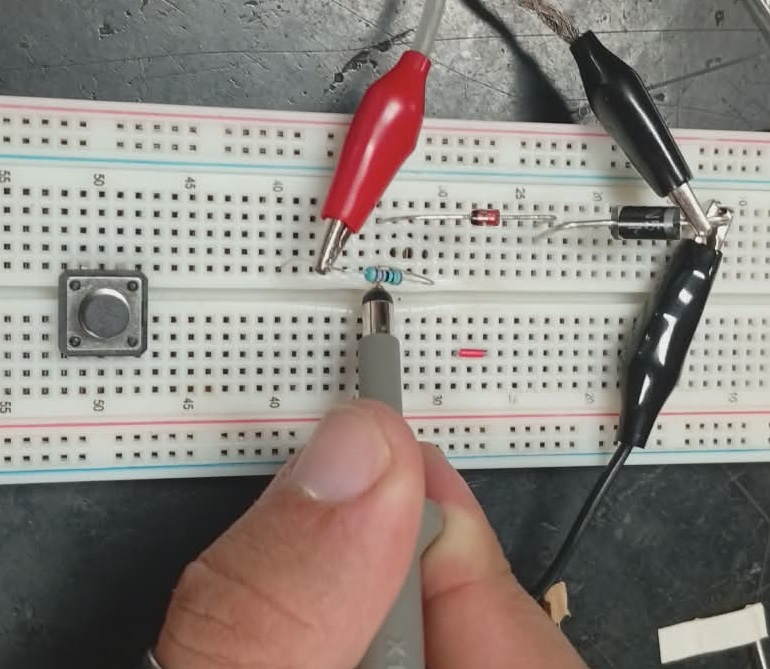
\includegraphics[height=6cm]{img/recotadores-con-zener2-protoboard.png}
    \caption{"modelo 2",Sección 3.4.1}
\end{minipage}
\hspace{0.02\textwidth}
\begin{minipage}{0.45\textwidth}
    \centering
    \includegraphics[height=6cm]{img/osciloscopio2.jpeg}
    \caption{Señal recortada }
\end{minipage}
\end{figure}


A partir de la simulación realizada, se verifica el comportamiento estudiado en la Sección~3.4, donde se analizó el funcionamiento de los circuitos recortadores con diodos Zener. 

Puede observarse que la señal de salida $V_0$ queda limitada aproximadamente a los valores determinados por las tensiones Zener de los diodos utilizados, produciendo el recorte
 de la señal sinusoidal de entrada.

